\documentclass[11pt]{beamer}
\usetheme{Madrid}
\usepackage[utf8]{inputenc}
\usepackage{amsmath}
\usepackage{amsfonts}
\usepackage{amssymb}
\usepackage{graphicx}
\usepackage{amsrefs}
\usepackage{algorithm}
\usepackage{algorithmic}
\usepackage{bbm}
\usepackage{subfigure}


\DeclareMathOperator {\argmin}{argmin}

\author{Hongda Li}
\title[MHC and SA]{Metropolis Hasting Chain and Simulated Annealing}
% Informe o seu email de contato no comando a seguir
% Por exemplo, alcebiades.col@ufes.br
\newcommand{\email}{email}
%\setbeamercovered{transparent}
\setbeamertemplate{navigation symbols}{}
%\logo{}
\institute[]{UBC Okanagan}
\date{\today}
%\subject{}

% ---------------------------------------------------------
% Selecione um estilo de referência
\bibliographystyle{plain}

%\bibliographystyle{abbrv}
%\setbeamertemplate{bibliography item}{\insertbiblabel}
% ---------------------------------------------------------

% ---------------------------------------------------------

\begin{document}

\begin{frame}
    \titlepage
\end{frame}

\begin{frame}{ToC}
    \tableofcontents
\end{frame}

\section{Introduction}

    \begin{frame}{The MHC}
        \begin{block}{MHC: Metropolis Hasting Chain}
            \begin{algorithmic}[H]
                \STATE{\textbf{Input: $X^{(t)}$}}
                \STATE{$Y^{(t)} \sim q (\cdot | X^{(t)})$}
                \STATE{
                    $ 
                    \rho(x, y) := 
                    \min\left\lbrace
                        \frac{f(y)}{f(x)}\frac{q(x|y)}{q(y|x)}, 1
                    \right\rbrace
                    $ 
                }
                \STATE{
                    $
                    X^{(t + 1)} := 
                    \begin{cases}
                        Y^{(t)} & \text{w.p}:  \rho(X^{(t)}, Y^{(t)})
                        \\
                        X^{(t)} &  \text{else}
                    \end{cases}$
                }
            \end{algorithmic}
        \end{block}
        \begin{itemize}
            \item [1.] $q(x|y)$ is doubly stochastic. 
            \item [2.] $f(x)$ is a distribution function up to a constant. 
            \item [3.] Must have $f(X^{(t)}) > 0$. 
        \end{itemize}
    \end{frame}
    \begin{frame}{What it does}
        Let $X^{(t)}$ be a sequence of observations sampled from the MHC, then $X^{(t)}$ will approximate $f$. 
        \begin{itemize}
            \item [1.] No integrals are needed. 
            \item [2.] It works very well for distribution functions in a very high dimension. 
            \item [3.] It is not hard to implement it on a computer. 
        \end{itemize}
    \end{frame}
    \begin{frame}{Primary questions}
        We have questions: 
        \begin{itemize}
            \item Is $f$ a stationary distribution for the MHC? 
                \begin{itemize}
                    \item Yes. 
                \end{itemize}
            \item Does it converge to the stationary distributions $f$? 
            \begin{itemize}
                \item Sometimes. We need some regularity conditions. 
            \end{itemize}
        \end{itemize}
        \vspace{2em}
        To converge to $f$ the MHC must satisfy the following: 
        \begin{itemize}
            \item [1.] $f$ is a stationary distribution of the MHC. 
            \item [2.] All states in $\text{supp}(f)$ can be commuted with each other. (f-Irreducible)
            \item [3.] The MHC is aperiodic. 
        \end{itemize}
    \end{frame}
    \begin{frame}{The transition kernel}
        \begin{block}{The transition kernel for MHC}
            \begin{align*}
                K(x, y) = 
                \rho(x, y)q(y|x) + 
                \left(
                    1 - \underbrace{\sum_{z \in S\setminus \{y\} }^{}\rho(x, z)q(z|x)}_{=:r(x)}
                \right) \mathbbm 1\{y = x\}. 
            \end{align*}
        \end{block}
        \begin{itemize}
            \item [1.] When $q$ is doubly stochastic, $f$ satisfies detail balance. ($f$-stationary)
            \item [2.] We have $K(x,x)> 0$ for all $x$ such that $f(x) > 0$. It is aperiodic. 
            \item [3.] It is f-irreducible if we assume $q(x|y)$ is non-negative for all $x, y\in \text{supp}(f)$. 
            \item [4.] See Robert and Casella's book \cite{book:robert_casella_2005} for the case where state space is continuous. 
        \end{itemize}
    \end{frame}
    \begin{frame}{Regularity conditions}
        \begin{itemize}
            \item [1.] $X^{(t)}$ needs to be able to travel to all states in $x\in \text{supp}(f)$. 
            \item [2.] And this is possible if $q(x|y) > 0 \;\forall x, y\in S$. 
            \item [3.] Weaker conditions exist, and we might have to do that in a case-by-case basis. We need to have: 
        \end{itemize}
        \begin{align*}
           \forall x,y \in \text{supp}(f) \;\exists n < \infty: K^n(x, y) > 0. 
        \end{align*}
    \end{frame}

\section{Numerical experiments, sampling}
    \begin{frame}{Sampling}
        The function we are sampling is: 
        \begin{align*}
            D &:= \{(x_1, x_2): -\sin(4\pi x_1) + 2\sin(2\pi x_2)^2 > 1.5\}
            \\
            f(x) &:= \mathbbm 1_D (\sin(x_14\pi) + \cos(x_24\pi) + 2), 
        \end{align*}
        on $[0, 1]\times [0, 1]$, and we are considering two choices of base chain: 
        \begin{itemize}
            \item [1.] A uniform random base chain, where it is just a random jump, is not a Markov chain. 
            \item [2.] A wrapped Guassian random walks, where $Y^{(t + 1)} \sim \text{WrappedNormal}(X^{(t)}, 0.1)$. (Or equivalently, Guassian random walks but with periodic boundary conditions.)
        \end{itemize}
    \end{frame}
    \begin{frame}{The sampling results}
        \begin{figure}
            \centering
            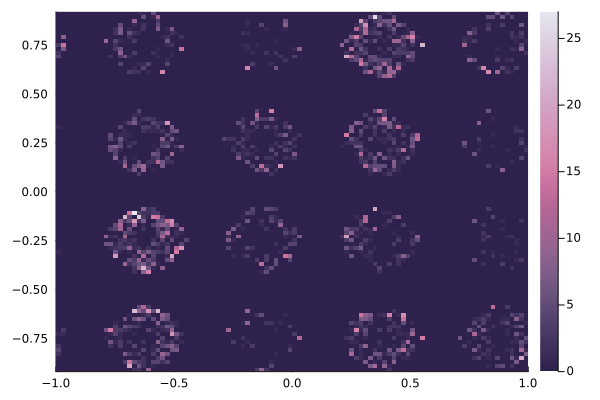
\includegraphics[width=3.5cm]{gaussian_base(1).png}
            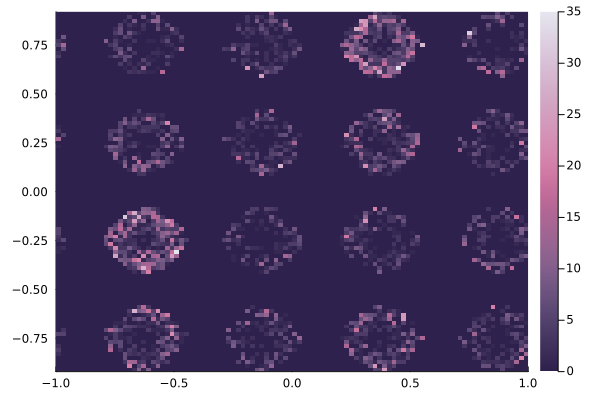
\includegraphics[width=3.5cm]{gaussian_base(2).png}
            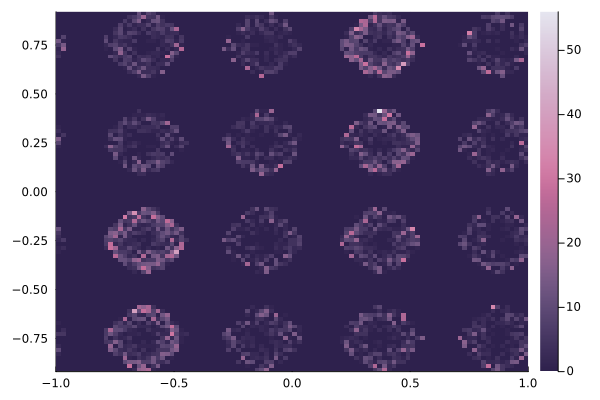
\includegraphics[width=3.5cm]{gaussian_base(3).png}
            \caption{Snapshots of accumulated samples when a wrapped Gaussian random walk base chain. The sampling is not quite even. }
            \label{fig:gaussian_rand_bc}
        \end{figure}
    \end{frame}
    \begin{frame}{The sampling results}
        \begin{figure}[h]
            \centering
            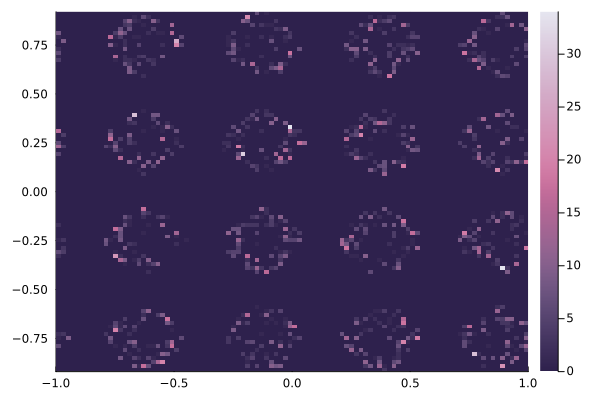
\includegraphics[width=3.5cm]{uniform_base(1).png}
            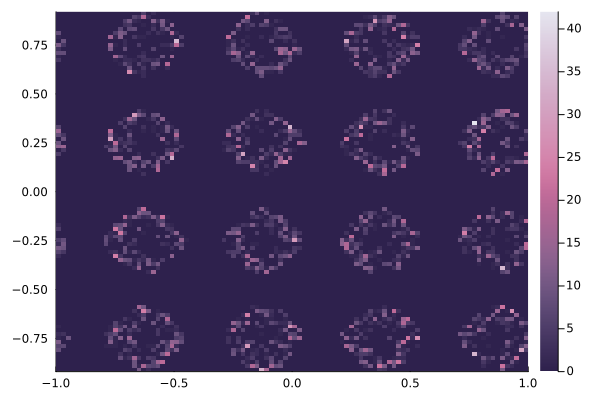
\includegraphics[width=3.5cm]{uniform_base(2).png}
            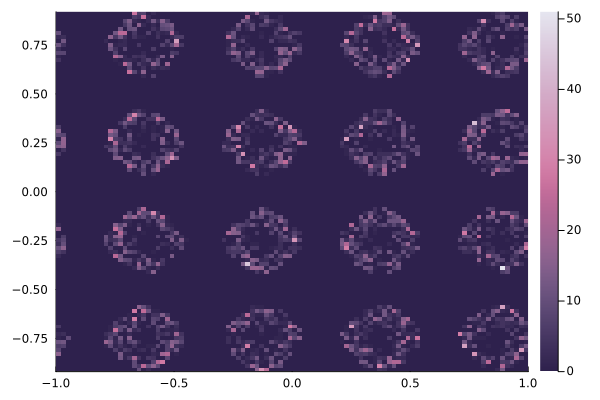
\includegraphics[width=3.5cm]{uniform_base(3).png}
            \caption{Snapshots of the accumulated samples when a uniform random base chain over $[0, 1]\times [0, 1]$. The sampling is quite even.} 
        \end{figure}
    \end{frame}
    \begin{frame}{Brief summary}
        \begin{itemize}
            \item [1.] It converges slowly if the base chain can not make $X^{(t)}$ travel from anywhere to everywhere. 
            \item [2.] The uniform base chain with an indicator function is the same Monte Carlo method. 
            \item [4.] If $\text{supp}(f)$ are disconnected, we need a base chain $q$ that is ``aggressive'' enough to make the jump, keeping MHC f-irreducible. 
            \item [5.] A combination of both is the key to efficiency. (In practice, we add these 2 base chains together, weighted by positive constants)
        \end{itemize}
    \end{frame}
\section{Simulated Annealing and Optimizations}
    \begin{frame}{Simulated Annealing}
        MHC can be used to maximizes $g: S\mapsto \mathbb R\cup \{-\infty\}$ through $f(x) = \exp(g(x)/T_i)$. $T_i$ is called a temperature. The lowering temperature accentuates the maximums of the function. Let $X^{*}$ denotes he set of maximizers for $f$ then as temperature goes to $0$, $f$ has: 
        \begin{align*}
            \lim_{i\rightarrow \infty}f(x) 
            &= 
            \lim_{i\rightarrow \infty} \frac{\exp(g(x)/T_i)}
            {
                \sum_{y\in S}^{}
                \exp(g(y)/T_i)
            }
            \\
            &= 
            \lim_{i\rightarrow \infty}
            \frac{1}{\sum_{y\in S}^{}\exp(g(y) - g(x)/T_i)}
            \\
            &= 
            \lim_{i\rightarrow \infty}
            \frac{1}{\exp(0) + \sum_{y\in S\setminus\{x\}}^{}\exp(g(y) - g(x)/T_i)}
            \\
            &= 
            \lim_{T\rightarrow 0}
            \frac{1}{1 + \sum_{y\in S\setminus\{x\}}^{}\exp(g(y) - g(x)/T)}
            \\
            &= \mathbbm 1\{X^*\}. 
        \end{align*}
    \end{frame}    
    \begin{frame}{Temperature illustrations}
        Let's make $g(x):= \text{sinc}(x)$ and plot with different temperatures: 
        \begin{figure}[h]
            \centering
            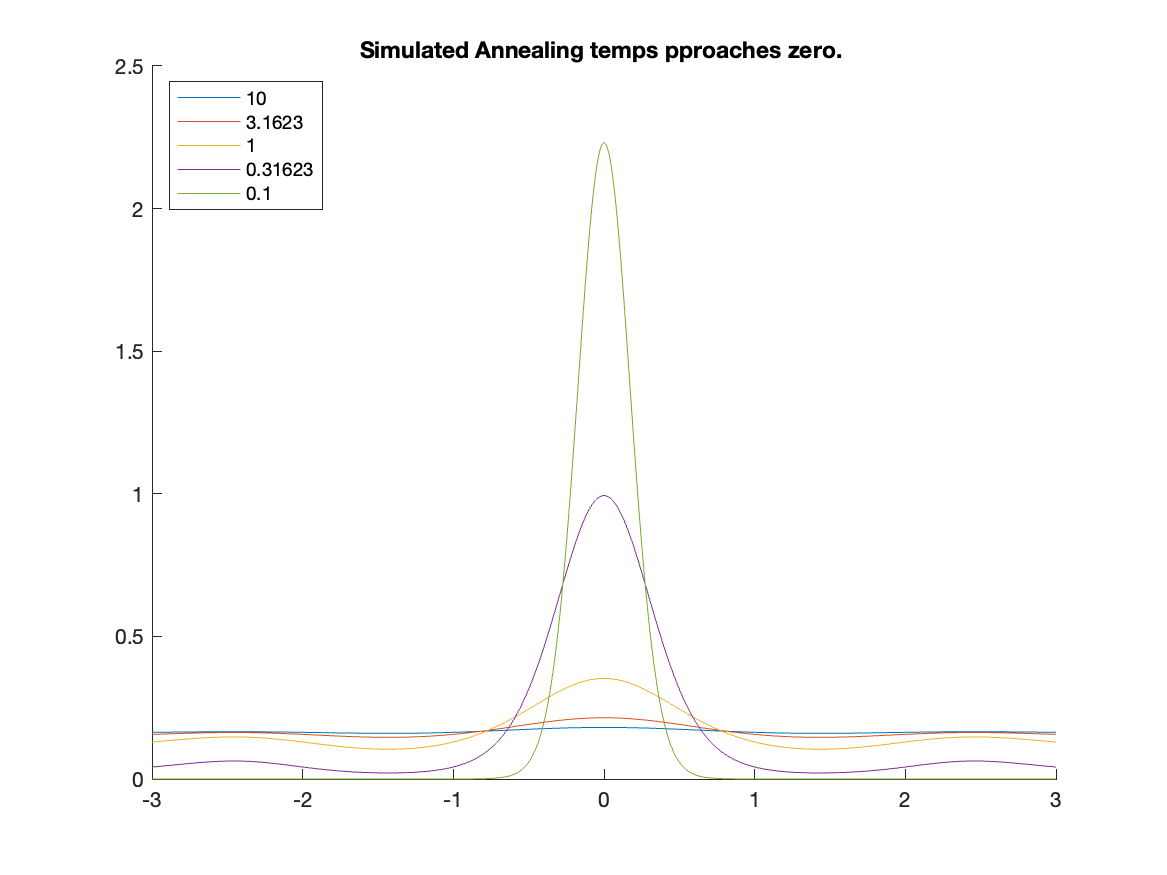
\includegraphics[width=8cm]{sa_temp.png}
            \caption{Different temperature when $g(x) = \text{sinc}(x)$, and $f := \exp(g(x)/T_i)$. }
        \end{figure}
    \end{frame}
    \begin{frame}{Temperatures and questions}
        \begin{itemize}
            \item [1.] Temperature helps with the convergence of Simulated annealing. As it gets lower, the MHC is more and more likely to reject sub-optimal solutions. Making it converges to a local optimal. 
            \item [2.] How would one choose the cooling schedule? 
            \item [3.] On top of all these, the choice of base chain is still a concern. 
        \end{itemize}
    \end{frame}
    \begin{frame}{Knapsack problem}
        Knapsack problem finds subsets from a given set such that it sums up as close to $1$ as possible while still having it less than $1$. It is phrased as: 
        \begin{align*}
            g(x) &:= \begin{cases}
                \langle w, x\rangle & \text{if }\langle w, x\rangle\le 1,
                \\
                -\infty & \text{else}. 
            \end{cases}
            \\
            f(x) &:= \exp(g(x)/T_i)
            \\
            S &:= \{0, 1\}^n. 
        \end{align*}
        The first 100 elements of $w$ sum up to 1 exactly, but the next 100 elements are sampled from $\sim \text{Uniform}(1, 2)$. 
    \end{frame}
    \begin{frame}{Temperatures}
        Using the base chain that mutates precisely one bit and flips that bit in $x$, we can avoid the curse of dimensionality. We consider the following three types of temperature schedules for our experiment: 
        \begin{itemize}
            \item [1.] The temperature drops quadratically from 1 to 0.001 every 1000 iterations, 10k iterations in total. 
            \item [2.] The temperature is $exp(-k)$ where k goes from 0 to 10. It decreases every 1000 iterations in a total of 10k iterations. 
            \item [3.] The temperature is $1/k^2$; it drops whenever the algorithm discovers a solution lower than all previous solutions for the objective function.
        \end{itemize}
    \end{frame}
    \begin{frame}{Numerical experiments results}
        \begin{figure}
            \centering
            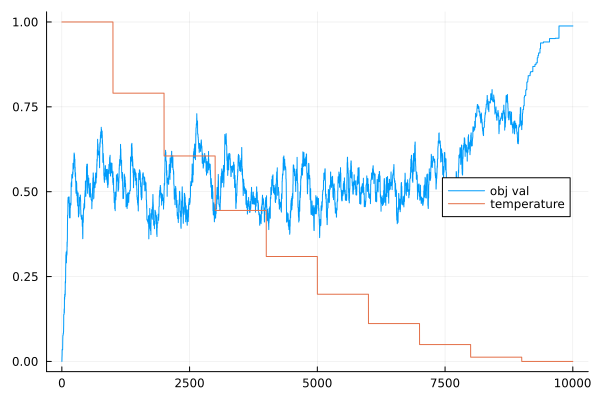
\includegraphics[scale=0.4]{sa_experiment1.png}
            \caption{Quadratic temperature schedule. }
        \end{figure}
    \end{frame}
    \begin{frame}{Numerical experiments results}
        \begin{figure}
            \centering
            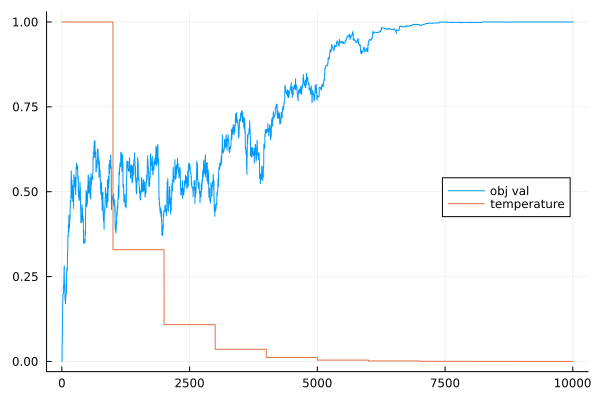
\includegraphics[scale=0.4]{sa_experiment2.png}
            \caption{Exponential temperature schedule. }
        \end{figure}
    \end{frame}
    \begin{frame}{Numerical experiments results}
        \begin{figure}
            \centering
            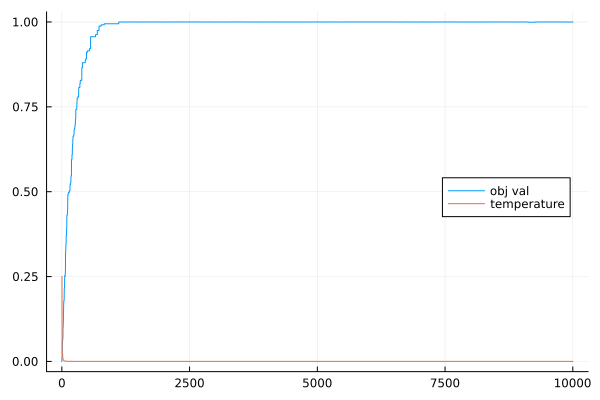
\includegraphics[scale=0.4]{sa_experiment3.png}
            \caption{Automatic temperature schedule. }
        \end{figure}
    \end{frame}
    \begin{frame}{Conclusion}
        \begin{itemize}
            \item Simulated Annealing makes a few assumptions, but at the same time, it is finicky, and the efficiency depends on many factors. These factors include: 
                \begin{itemize}
                    \item underlying structure of the problem. 
                    \item properties of the feasible region (Disconnected? Measurable?).
                    \item temperature schedule. 
                    \item base chain (is it going to be cursed by dimensionality? does it achieve f-irreducibility?). 
                \end{itemize}
            \item It is relatively easy to implement and is trivial to parallelize on a modern computer. 
            \item In general, it can find the local optimal, but it might not be able to find the global optimal. 
        \end{itemize}
    \end{frame}

\section{References}
    \begin{frame}{References}
        \bibliography{refs.bib}
    \end{frame}

\end{document}